\section{Simulation Analysis}
\label{sec:simulation}

The circuit used to simulate the output impedance of the amplifier as a whole was the one that can be found in the following figure. The intermediate input and output impedances for the different stages were not simulated.

\begin{figure}[H] \centering
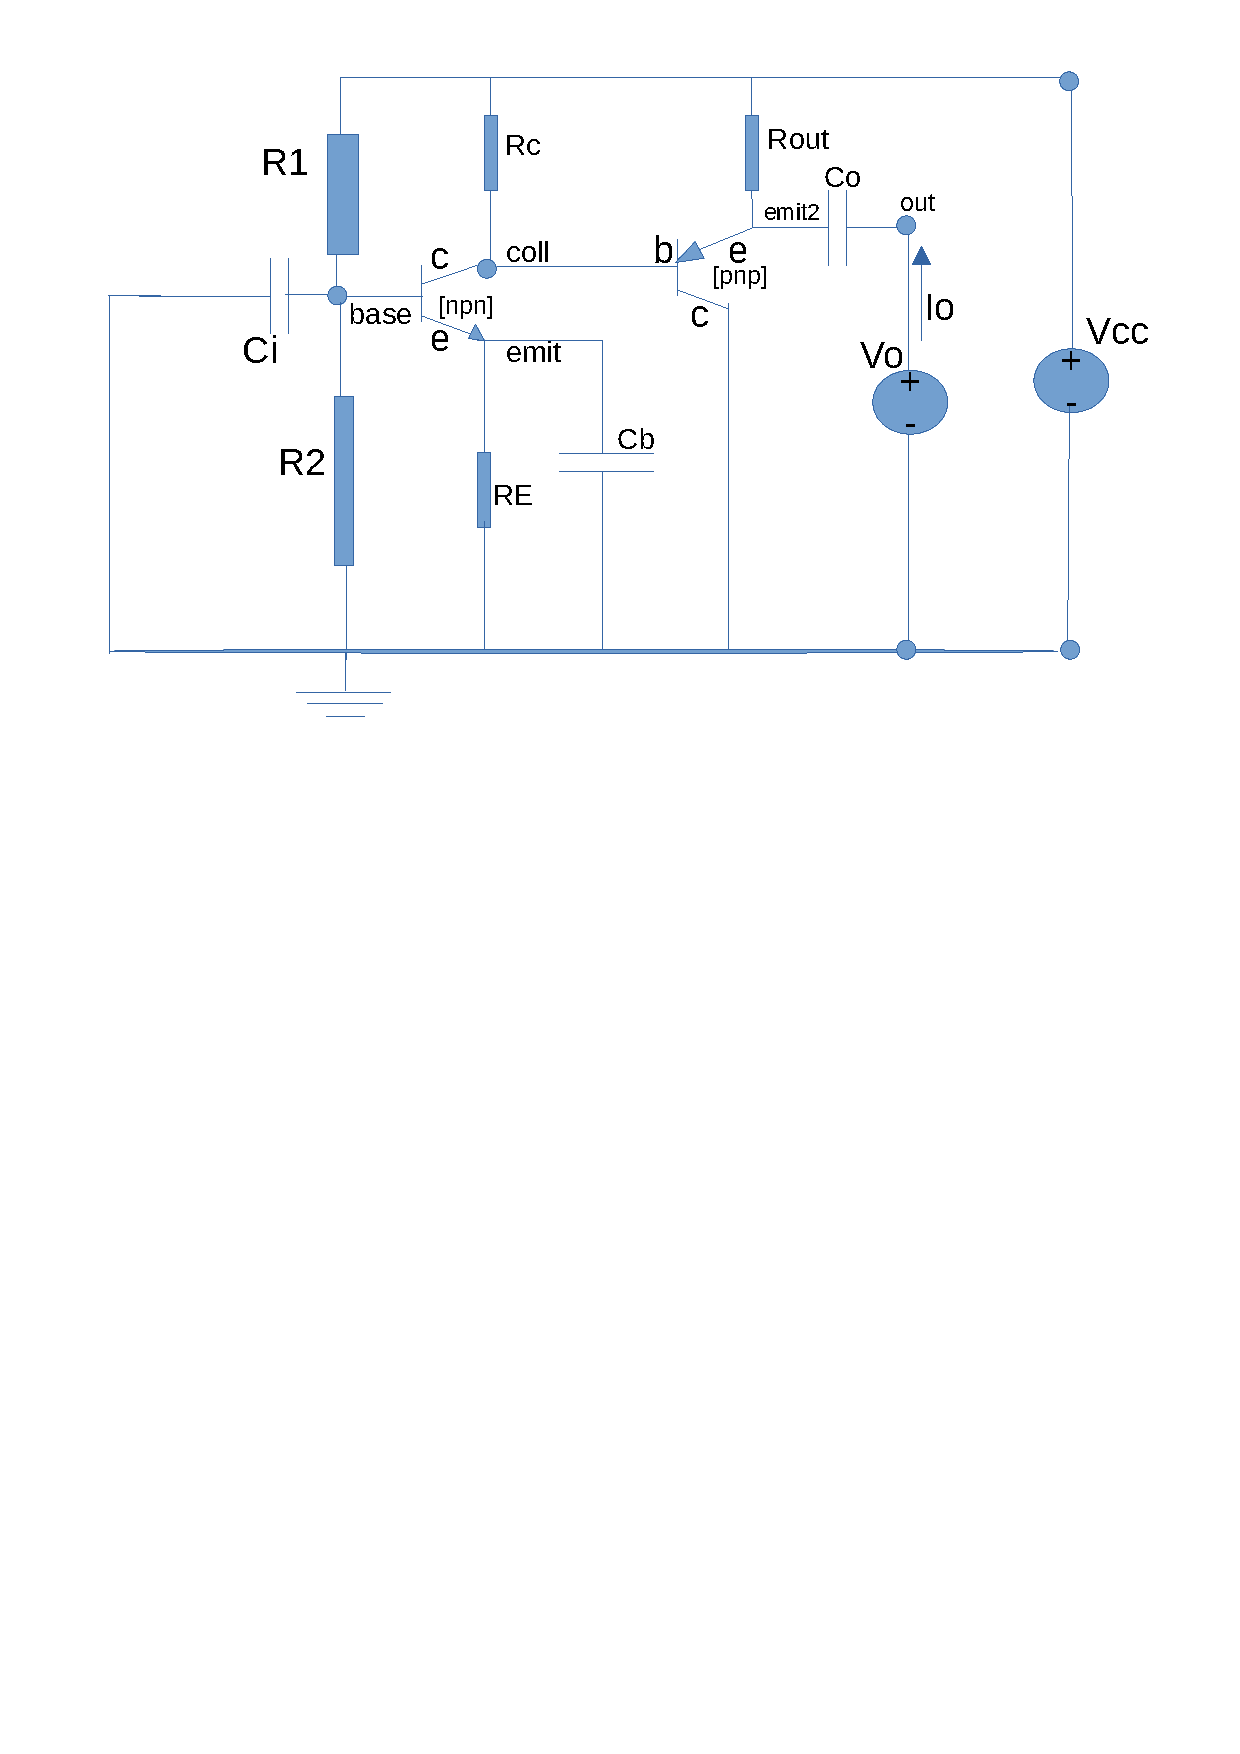
\includegraphics[width=0.95\linewidth]{diagram_t4_zout.pdf}
\vspace{-10cm}
\caption{Diagram of the circuit considered for the simulation of the output impedance of the amplifier .}
\label{fig:diagram_t4_zout}
\end{figure}


The gain of the audio amplifier, the upper and lower cut off frequency, the bandwidth and the input and output impedances as well as the merit are presented in the following table, both for the theoretical analysis (right) and for the Ngspice simulation (left), in order to make a side-by-side comparison.

\hfill
 \parbox{1\linewidth}{
  \centering
  \begin{tabular}{|l|l|l|r|}
    \hline    
    {\bf Parameter} & {\bf Simulation} & {\bf Theoretical } & {\bf Units }\\ \hline
    $Zi_{total}$ & 385.039 & 283.57 & Ohm\\ \hline
$Zo_{total}$ & 4.00907 & 2.8721 & Ohm\\ \hline
$Zi_{gain}$ & - & 283.57 & Ohm\\ \hline
$Zo_{gain}$ & - & 191.47 & Ohm\\ \hline
$Zi_{output}$ & - & 31066.9 & Ohm\\ \hline
$Zo_{output}$ & - & 2.0552 & Ohm\\ \hline
Cost & 6090.8 & 6090.8 & MU\\ \hline
uco & 4254308.000 & 4254308.000 & Hz\\ \hline
lco & 20.540 & 84.305 & Hz\\ \hline
Bandwidth & 4254287.460 & 4254223.695 & Hz\\ \hline
$Gain_{gainstage}$ & - & 87.937 & [adimensional]\\ \hline
$Gain{outputstage}$ & - & 0.985 & [adimensional]\\ \hline
$Gain{total}$ & 39.575 & 86.592 & [adimensional]\\ \hline
MERIT & 1345.8247 & 717.4149 & gold medals\\ \hline

  \end{tabular}
  \label{tab:results}
    %\caption{Side-by-side comparison of the circuit parameters (resistors, capacitors, etc) and the corresponding results (ripple, average, merit)}
  }

  

\subsection{Output voltage gain in the passband}
\par
\vspace{-4cm}
\begin{figure}[H] \centering
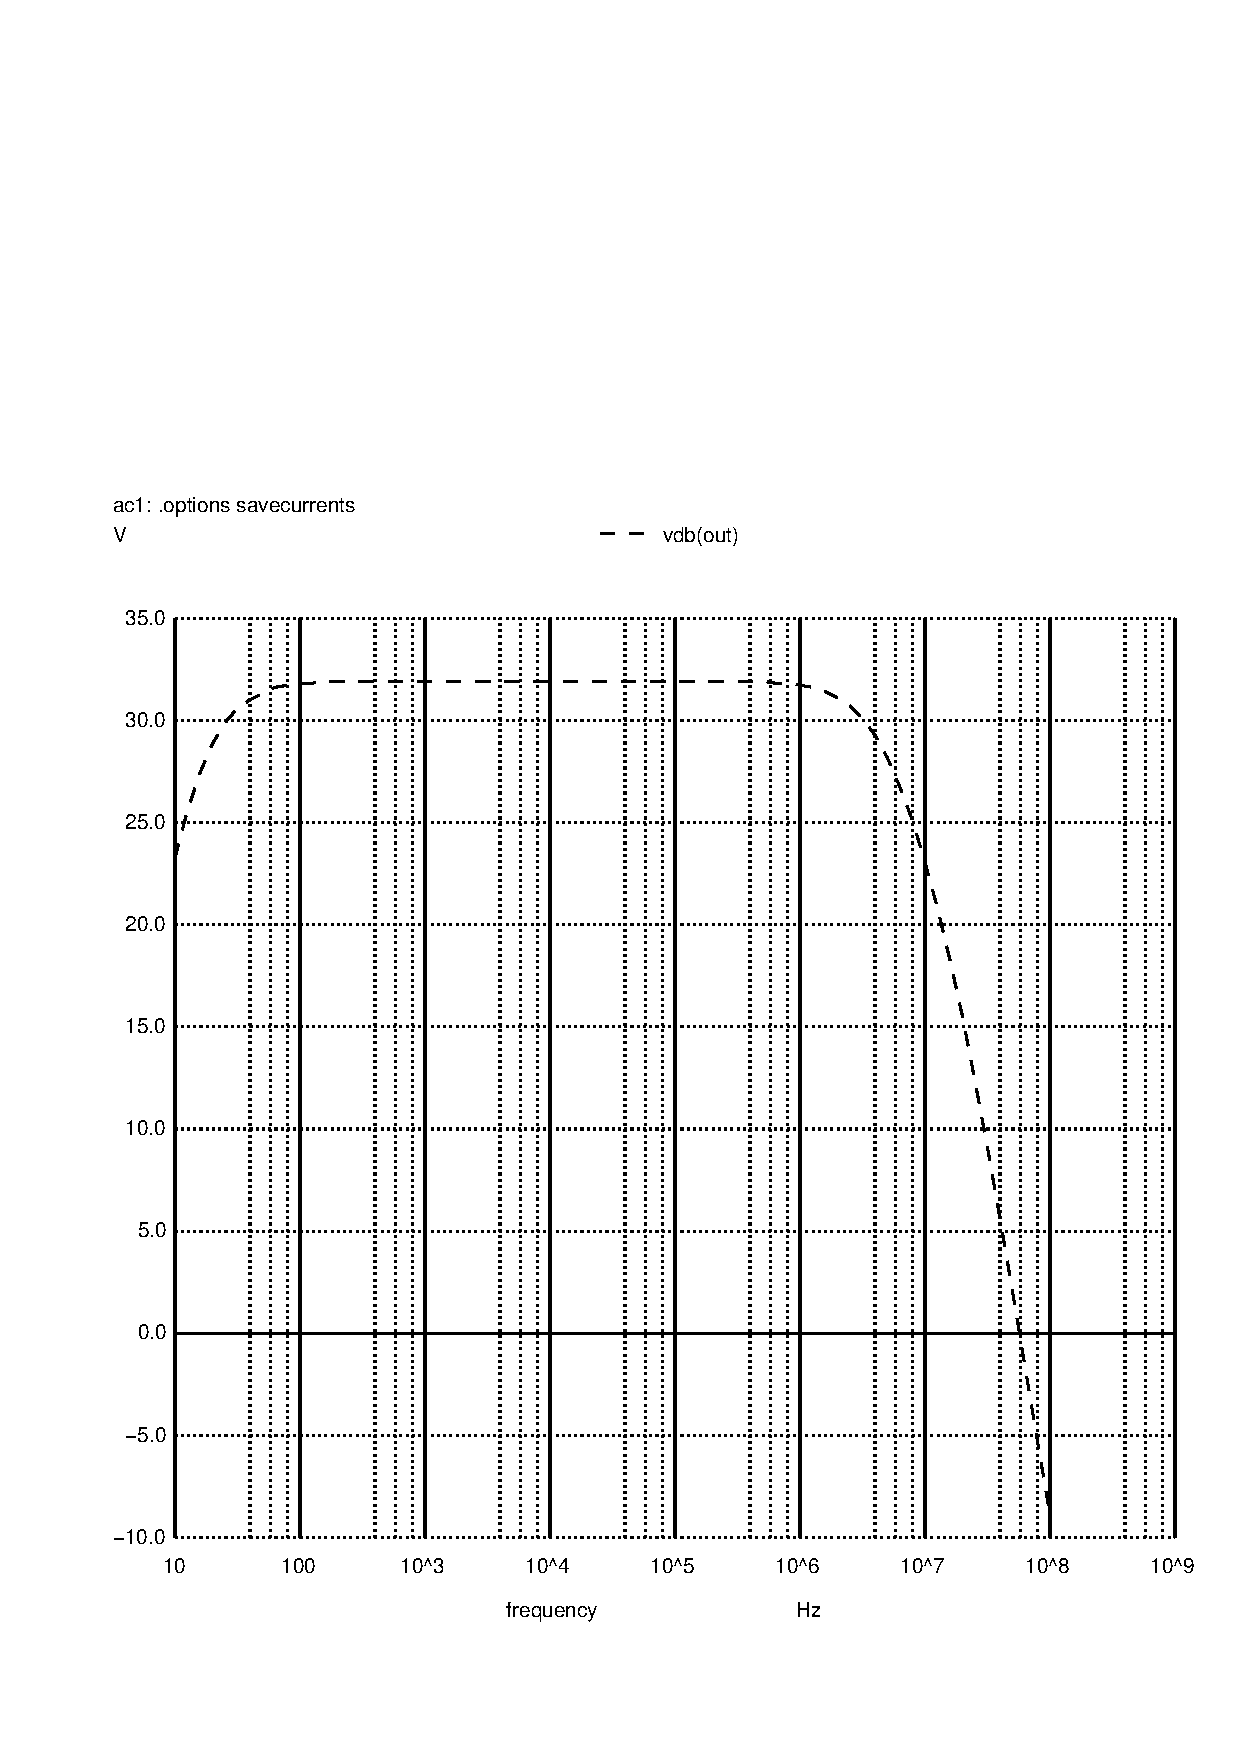
\includegraphics[width=0.6\linewidth]{vo2f.pdf}
\vspace{-1cm}
\caption{Output voltage gain in the passband}
\label{fig:gain_sim}
\end{figure}


\subsection{The input and output impedances}

\begin{figure}[H] \centering
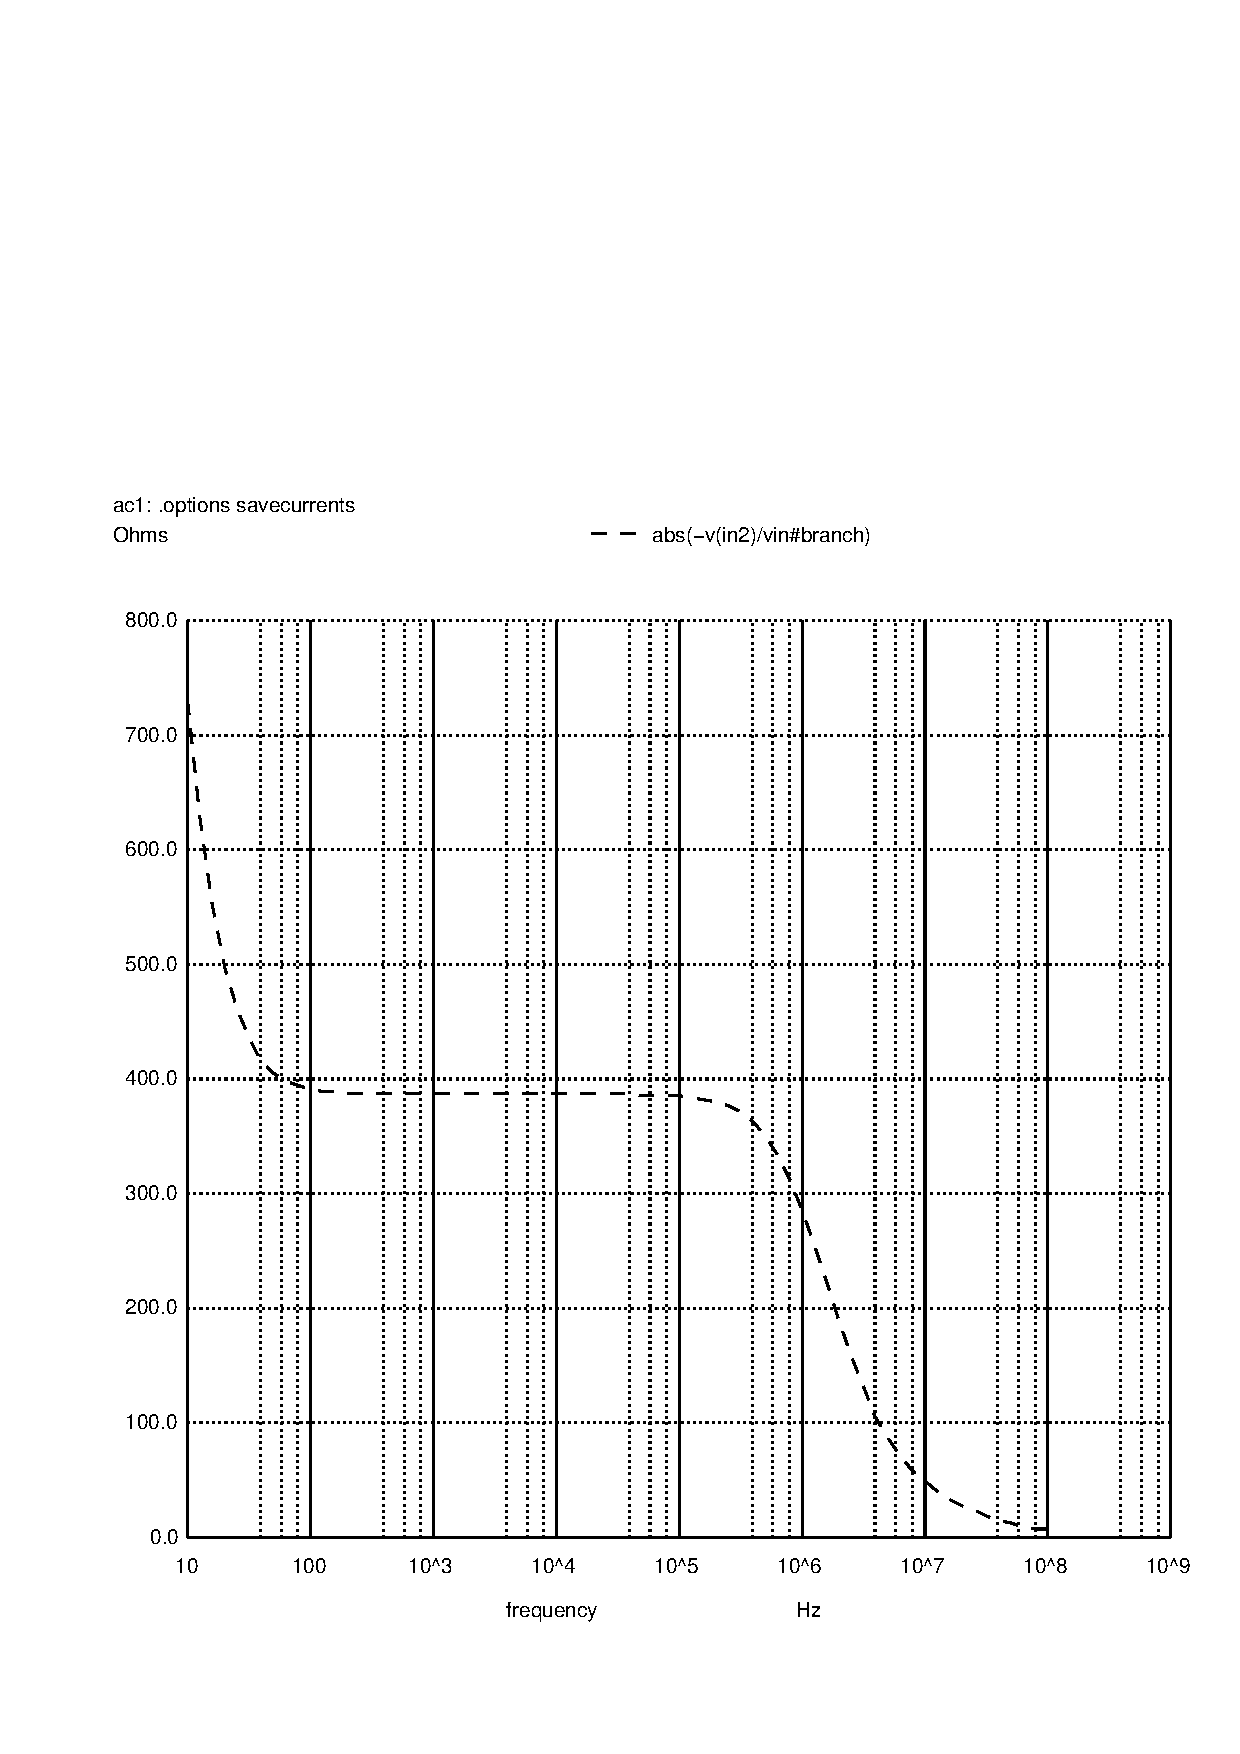
\includegraphics[width=0.6\linewidth]{zin.pdf}
\caption{Input impedance of the Audio amplifier circuit}
\label{fig:In_imp}
\end{figure}
\vspace{-3cm}


\begin{figure}[H] \centering
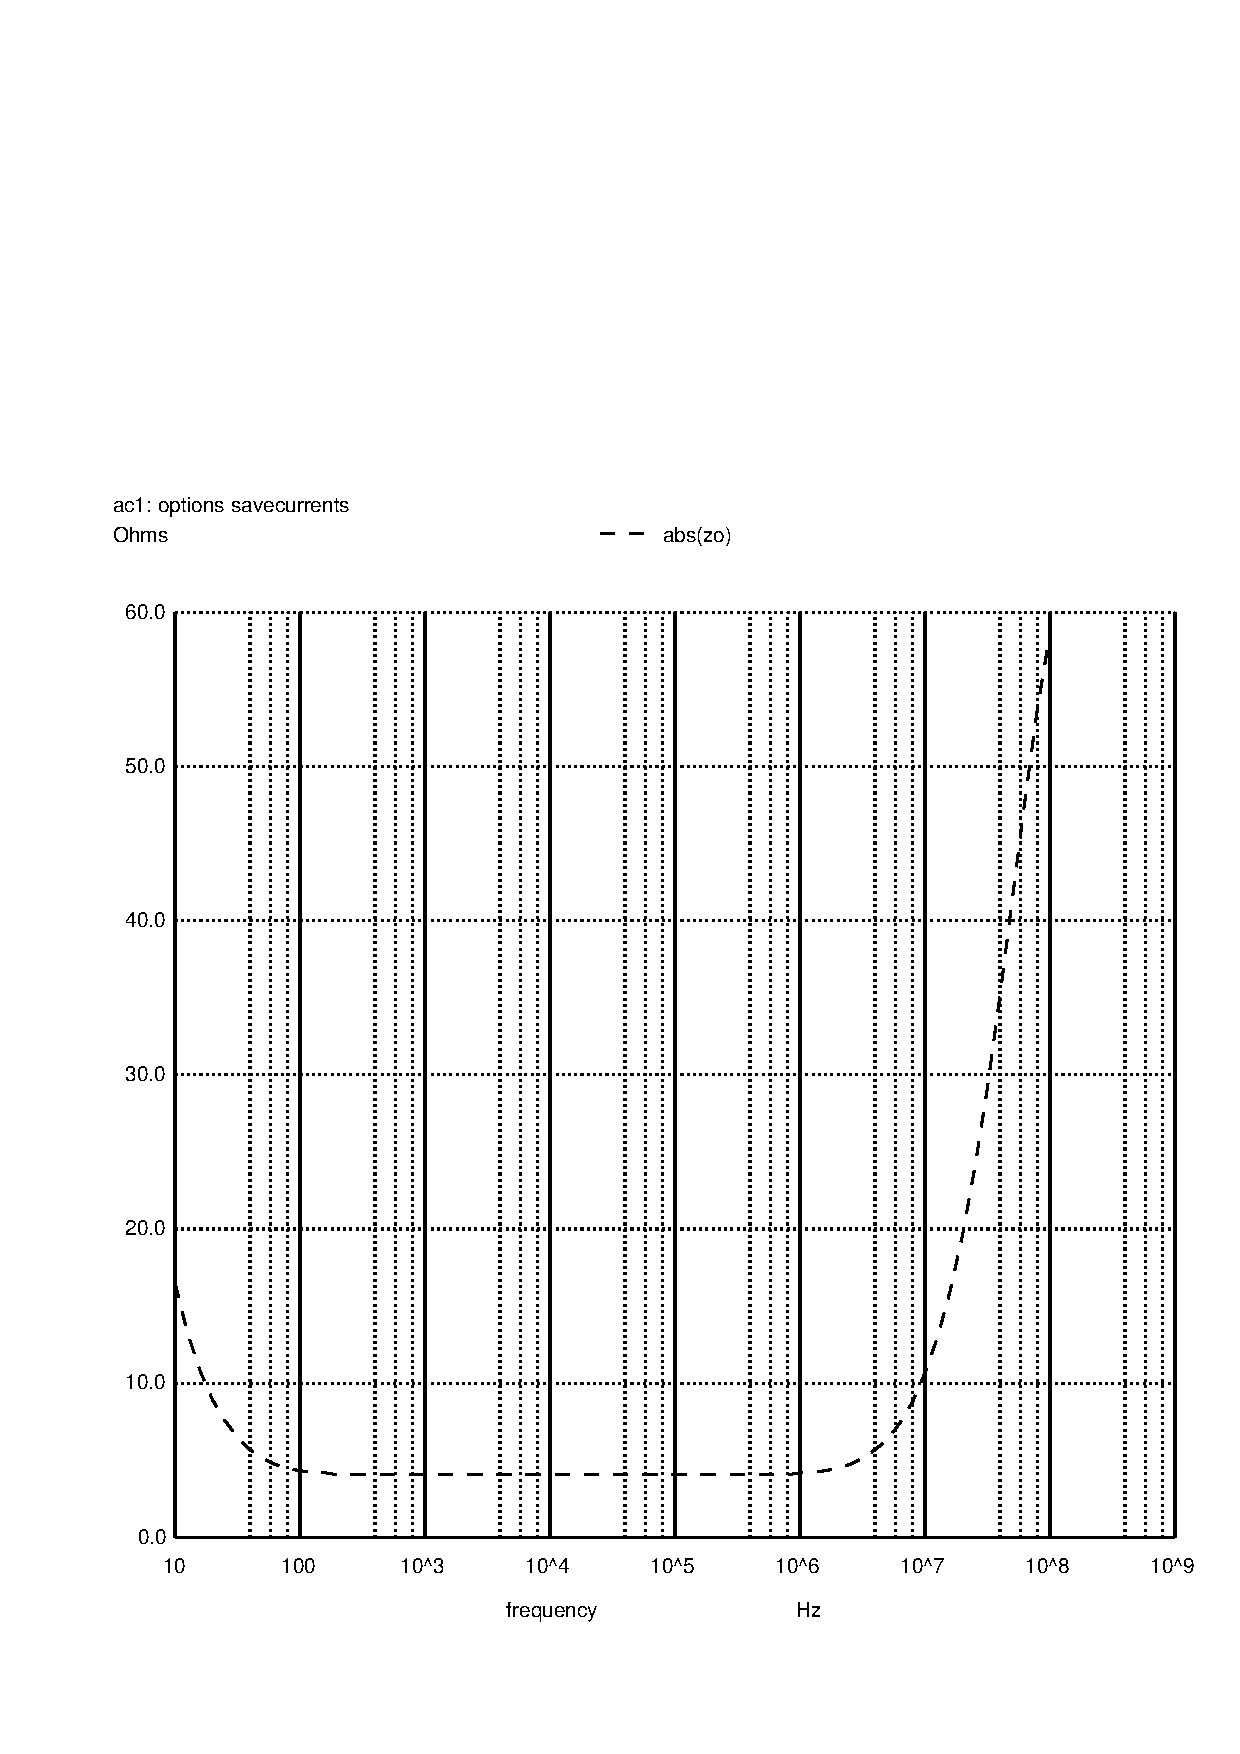
\includegraphics[width=0.6\linewidth]{zoinc.pdf}
\caption{Output impedance of the Audio amplifier circuit}
\label{fig:out_imp}
\end{figure}
\vspace{-3cm}


\pagebreak
